%===============================================================================
% Presentation
%===============================================================================
% $Id$
%===============================================================================


%===============================================================================
% Configuration
%===============================================================================


%-------------------------------------------------------------------------------
% \documentclass and \usepackage directives
%-------------------------------------------------------------------------------
\documentclass{beamer}
\usepackage{beamerthemebars}
\usepackage[english]{babel}
\usepackage[latin1]{inputenc}

% Compilation with latex or pdflatex?
\newif\ifpdf 
\ifx\pdfoutput\undefined 
  \pdffalse
\else
  \pdfoutput=1 
  \pdftrue 
\fi 

% Compilation with pdflatex
\ifpdf
 
  \usepackage[pdftex]{graphicx}

  \pdfinfo{
    /Title      (EiffelRSS Presentation)
    /Author     (Thomas Weibel, Martin Luder, Michael K�ser)
    /Subject    (Eiffel programming)
    /Keywords   (Programming, EiffelRSS)
  }

% Compilation with latex
\else 

  \usepackage{graphicx} 

\fi



%-------------------------------------------------------------------------------
% Use some nice templates
%-------------------------------------------------------------------------------
\beamertemplateshadingbackground{blue!10}{structure!10}
\beamertemplatetransparentcovereddynamic
\beamertemplateballitem
\beamertemplatenumberedballsectiontoc
\colorlet{beameralert}{blue!60!black}


%-------------------------------------------------------------------------------
% Configure \titlepage
%-------------------------------------------------------------------------------
\title{EiffelRSS}
\author{Martin Luder \and Michael K�ser \and Thomas Weibel}


%===============================================================================
% Document
%===============================================================================
\begin{document}


% Titlepage
\frame{
  \titlepage
}

\section{RSS}

\frame{
  \frametitle{What is RSS?}

  \begin{itemize}[<+-| alert@+>]
  \item Acronym for Really Simple Syndication, Rich Site Summary or
    RDF Site Summary
  \item XML format for syndicating news, the content of news-like
    sites and pretty much anything that can be broken down into
    discrete items, e.g. the "recent changes" page of a Wiki, a
    changelog of SVN checkins, even the revision history of a book
  \item Once information about each item is in RSS format, an
    RSS-aware program can check the feed for changes and react to the
    changes in an appropriate way.
  \item There are 9 different and incompatible versions of RSS,
    EiffelRSS handles only RSS 2.0 at the moment, but can handle all
    of them through specialized reader and writer classes.
  \end{itemize}
}


\section{Overview}

\frame{ 
  \frametitle{What is EiffelRSS?}

  \begin{itemize}[<+-| alert@+>]
  \item EiffelRSS is an Eiffel library to read and write RSS. The goal
    is to provide the Eiffel development community with an easy to use
    and well structured API for RSS.
  \item The distribution also contains a RSS newsfeed reader written
    with EiffelVision and EiffelRSS.
  \end{itemize}
}


\section{Library}

\frame{
  \frametitle{EiffelRSS Library: Helper Clusters}
  
  \begin{itemize}[<+-| alert@+>]
  \item \texttt{ADT} features classes to implement sortable
    structures.
  \item \texttt{FETCH} can fetch data from a source address to a local
    \texttt{STRING} using HTTP, FTP and file.
  \item \texttt{LOGFILE} represents a file which can be used for
    logging messages during the program execution.
  \item \texttt{PROPERTIES} represents a persistent set of properties.
  \end{itemize}
}

\frame{
  \frametitle{EiffelRSS Library: SYNDICATION}

   \begin{itemize}[<+-| alert@+>] 
   \item \texttt{SYNDICATION} is the main cluster of EiffelRSS with a
     feed object model, and classes to load and write feeds. It has
     three subcusters:
        \begin{itemize}
        \item \texttt{INTERFACE} contains all the classes a developer
          needs to use the library.
        \item \texttt{FEED} is the central datastructure of EiffelRSS.
          It defines an abstract syndication feed.
        \item \texttt{FORMATS} defines the different syndication
          formats. It is easy extensible with other formats.
        \end{itemize}
  \end{itemize}
}

\frame{
  \frametitle{EiffelRSS Library: SYNDICATION}

  \begin{center}
    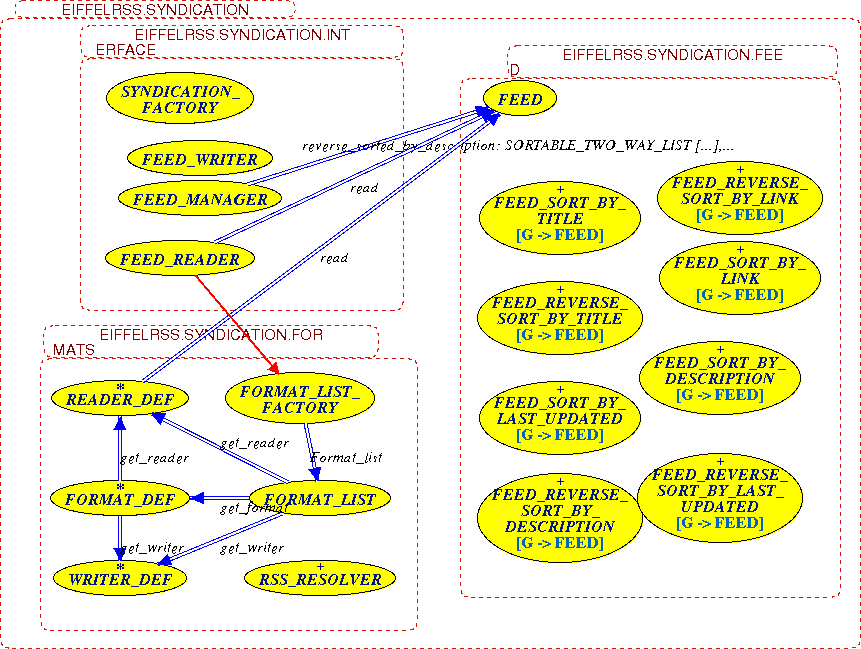
\includegraphics[scale=.3]{figures/EIFFELRSS_SYNDICATION}
  \end{center}
}

\section{Newsreader}

\frame{
  \frametitle{EiffelRSS newsreader}

  \begin{itemize}[<+-| alert@+>]
  \item Newsreader is a simple RSS-feed reader which shows the
    possibilities of the EiffelRSS library.
  \item You can add custom feeds and open news in your Internet
    browser.
  \item Features a graphical and command line user interface.
  \end{itemize}

  \begin{center}
    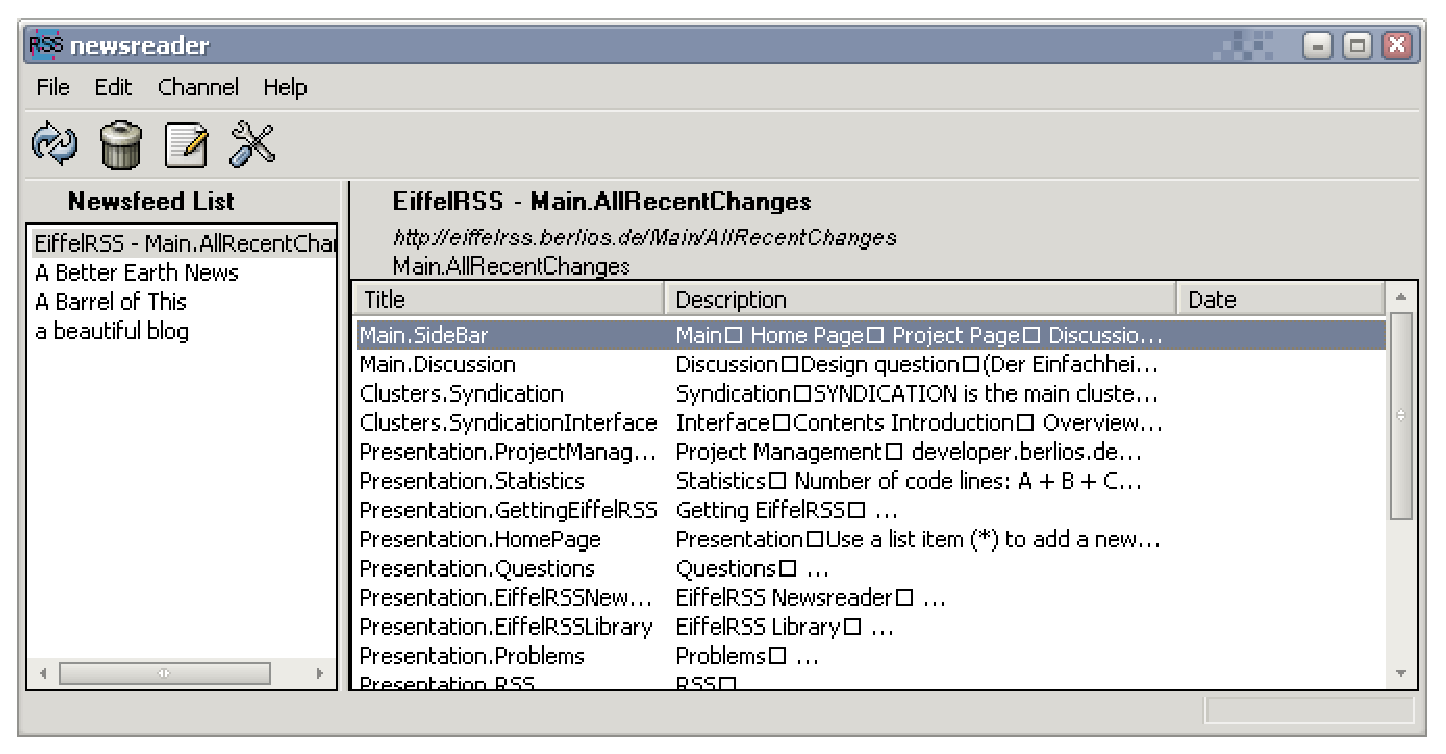
\includegraphics[scale=.3]{figures/newsreader}
  \end{center}
}


\section{Download}

\frame{
  \frametitle{Getting EiffelRSS}

  \begin{itemize}[<+-| alert@+>]
  \item http://eiffelrss.berlios.de
  \item Subversion: svn checkout svn://svn.berlios.de/eiffelrss
  \end{itemize}
}


\section{Project Management}

\frame{
  \frametitle{Project Management}

  \begin{itemize}[<+-| alert@+>]
  \item developer.berlios.de
  \item Subversion
  \item PmWiki
  \item Gobo Eiffel test (getest)
  \end{itemize}
}


\section{Problems}

\frame{
  \frametitle{Problems}

  \begin{itemize}[<+-| alert@+>]
  \item EiffelNet has only support for HTTP 1.0 and is quite unstable
  \item The XML parser of gobo has problems with entites and special characters
  \item No sortable data structures
  \item No real stream concept, e.g. input and output are no files
  \end{itemize}
}


\section{Statistics}

\frame{
  \frametitle{Statistics}

  \begin{itemize}[<+-| alert@+>]
  \item Number of Eiffel code lines: A + B + C
    \begin{itemize}
    \item Library: A
    \item Newsreader: B
    \item Examples and testing framework: C
    \end{itemize}
  \item Number of Eiffel classes: X + Y + Z
    \begin{itemize}
    \item Library: X
    \item Newsreader: Y
    \item Examples and testing framework: Z
    \end{itemize}
  \end{itemize}
}

\end{document}
